% Chapter Template

\chapter{Original Work} % Main chapter title

\label{Chapter3} % Change X to a consecutive number; for referencing this chapter elsewhere, use \ref{ChapterX}

\section{Outline}
The original work of \parencite{klampfl_maass_2013} that is replicated in this paper is based on the \textit{liquid computing model}. This computing paradigm is loosely inspired by biological brains and offers a way of implementing Spiking Neural Networks (SNNs). It consists of a collection of nodes (that resemble neurons) that can send and receive temporal signals (also called spikes) to and from other nodes via dedicated connections (which resemble synapses). These connections - just like the nodes - can have various other properties, such as delay or weight that influence how spikes are transmitted over the network of nodes. Additionally, neurons also possess a spatial coordinate that is necessary for having distance-dependent connection probabilities just like in the brain.\\
The conventional liquid computing model abstracts a fair amount of detail however, when compared to real cortical circuits. This includes a major structural trait inherent to the brain, that is assumed to enable long-term memory by forming stereotypical assemblies of neurons: synaptic plasticity. In the original paper, two forms of plasticity are used: short-term plasticity (STP) and spike-time dependent plasticity (STDP).\\
This chapter will first describe the initial structural setup of the network from the original implementation in Section \ref{sec:basic_network_structure} and then lay out how the generation and distribution of outside input is handled in Section \ref{sec:input_generation}. Finally, the dynamic properties that give the model its actual capabilities are discussed in Section \ref{sec:dynamic_network_behaviour}.

\section{Basic Network Structure} \label{sec:basic_network_structure} % including lateral inhibition
\begin{figure}[htbp]
  \centering
  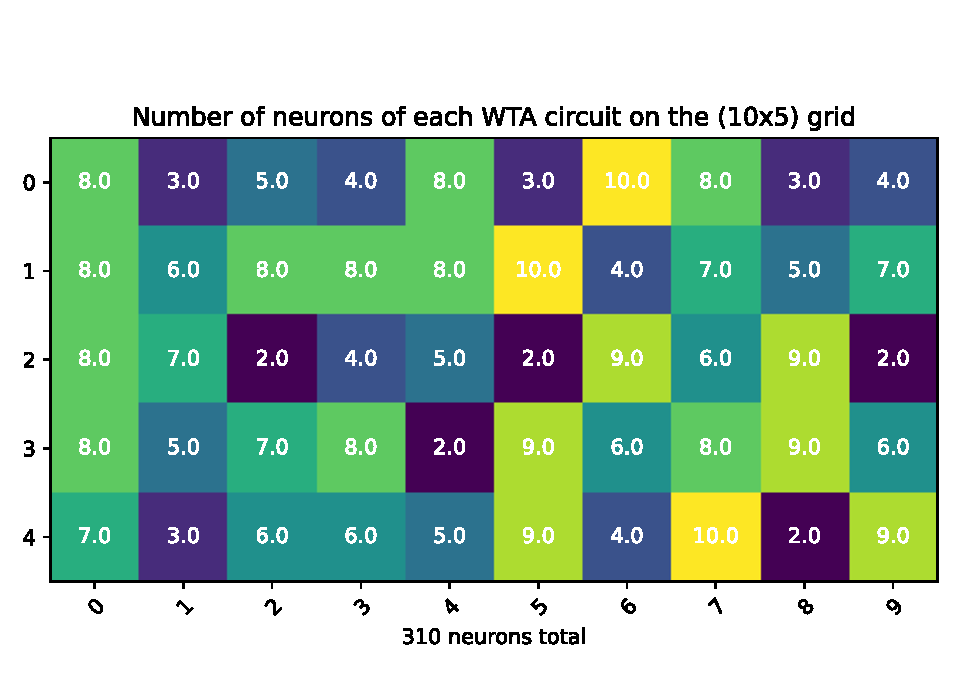
\includegraphics[width=0.9\columnwidth]{Figures/circuit_grid2D.pdf}
  \caption{Visualization of a random $10\times 5$ WTA circuit grid with $k_{min}=2, k_{max}=10$}
  \label{fig:circuit_grid}
\end{figure}
The basic setup of the liquid computing model employs a 2D grid of so-called Winner-Take-All (WTA) circuits, usually set to a size of $10\times 5$ as in the example grid in Figure \ref{fig:circuit_grid}. The 2D grid is utilized to assign spatial coordinates to each WTA, for the purpose of constructing inter-circuit connections with distance-dependent probability. The reason for this is that it has been found that in the brain, the probability that two neurons are synaptically connected decreases as their spatial distance increases. To describe this structural property mathematically, there exist multiple different rules including the following chosen for the original implementation:
\begin{equation}
    p(d)=\lambda e^{-\lambda d} \label{eqn:distance_dependent_probability}
\end{equation}
where $d$ is the euclidean distance between two WTA circuits and $\lambda$ is a generic setting parameter for adapting the connectivity rule to work well with the given grid size. In the original implementation $\lambda=0.088$.\\
The WTA circuits themselves are each composed of neurons $z_1, \dots, z_K$, where the integer $K$ is uniformly drawn at random from a range $[k_{\min}, k_{\max}]$. All neurons $z_1, \dots, z_K$ in the same WTA are not laterally connected and are subject to a mechanic called lateral inhibition. This is illustrated in Figure \ref{fig:wta_circuit}. Lateral inhibition causes that when one neuron in the WTA circuit fires, all other neurons in the same circuit experience inhibition, i.e. are discouraged from also firing. The biologically most accurate solution for implementing it would be to introduce inhibitory neurons that receive input from the entire WTA and output inhibitory spikes to the same circuit (as seen in Fig. \ref{fig:wta_circuit}).\\
In \parencite{klampfl_maass_2013} this is however said to be realized in a different way, by adjusting the firing rate of each neuron $k$ according to the summed firing rate of the WTA like this:
\begin{equation}
    r_k(t)=R_{\max}\cdot \frac{e^{u_k(t)}}{\sum_{j=1}^{K} e^{u_j(t)}}
    \label{eqn:firing_rate_paper}
\end{equation}
$R_{\max}$ is a fixed value that defines the maximum firing rate and is usually set to \SI{100}{\hertz}. $u_k(t)$ on the other hand stands for the current membrane potential of neuron $z_k$ at time $t$ and will be explained in more detail in Section \ref{sec:dynamic_network_behaviour}.
This realization of lateral inhibition bypasses the use of dedicated inhibitory neurons for lateral inhibition but is also responsible for normalizing the firing rate of the combined WTA circuit to $R_{\max}$, even when no external inputs are present. In principle, this is an unwanted side-effect, but according to \parencite{klampfl_maass_2013}, this is insignificant to the results of their study. Replacing this mode of lateral inhibition might be interesting for future work with the model from their paper.\\

\begin{figure}[htbp]
  \centering
  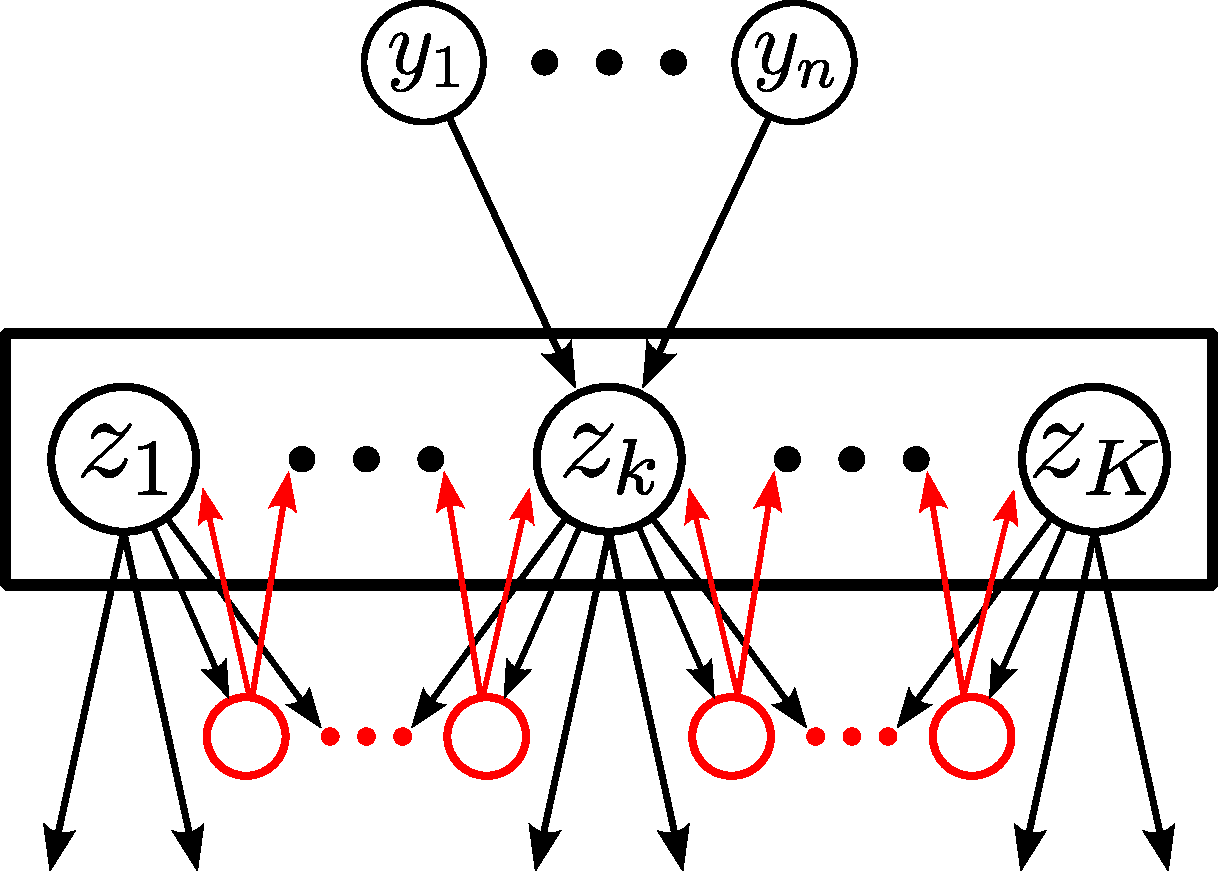
\includegraphics[width=0.8\columnwidth]{Figures/wta_circuit.pdf}
  \caption{WTA circuit with lateral inhibition}
  \label{fig:wta_circuit}
\end{figure}

\section{Running the Network} \label{sec:running_the_network}
The original model offers two different functions of running the network and producing readouts: \texttt{test()} and \texttt{simulate()}. The core difference is that during testing the network is not trained, i.e. the usual dynamic behavior resulting from STDP is disabled so that weights are not updated while running. STP is always enabled, while the use of variance tracking (described in Section \ref{sec:variance_tracking}) is optional but seems to be a requirement for learning with STDP, based on trials conducted with the original code. These findings are further discussed in Chapter \ref{Chapter5}.\\
Apart from the enabling of STDP, \texttt{test()} and \texttt{simulate()} are similar and share the same basic functionality. The network is run by progressing it step by step, where one step usually represents a time span of \SI{1}{\ms} (depending on the value of \texttt{dt}), after which the network states are updated according to the rules specified in Section \ref{sec:dynamic_network_behaviour}.

\section{Input Generation} \label{sec:input_generation}
To train the network properly for different tasks, the generation of input is key. In its simplest form, this is implemented as the presentation of recurrent pattern inputs, as illustrated in Figure \ref{fig:input_generator}. More complex sequences can also be generated based on this, but this will be briefly discussed in Chapter \ref{Chapter4} as it is not crucial for the tests performed in this thesis. The patterns here (represented by the grey boxes) consist of a number of input spike trains, where each input source gets its own Poisson spike train generated. Poisson generation is essentially realized by randomly sampling a list of values from an exponential distribution
\begin{equation}
    f(x;\frac{1}{\beta})=\frac{1}{\beta}\exp{\left(-\frac{x}{\beta}\right)},
    \label{eqn:exponential_distribution}
\end{equation} 
where $\beta$ corresponds to the firing rate in \SI{}{\hertz} of each spike train in that pattern. This list is then cumulatively summed, i.e. the list of values $v_1, \dots, v_k$ is updated as follows: $v_n\prime=\sum_{i=0}^{n-1} v_i$ to obtain an ascending list $v_1\prime, \dots, v_k\prime$ of spike times with interspike intervals (ISIs) drawn from Equation \ref{eqn:exponential_distribution}. This pattern generation has to be done once for every pattern before the network is run with pattern inputs.\\
These pattern inputs are however not the only kind of input that the network neurons receive. Unless disabled, they also receive random noise of frequency \texttt{rNoise} [\SI{}{\hertz}], which is constantly overlaid. The resulting two different types of total input can therefore be distinguished into noise and pattern phases of duration \texttt{tNoise} and \texttt{tPattern} respectively, where \texttt{tNoise} is uniformly drawn at random from the pre-specified interval \texttt{tNoiseRange}.\\
As already explained in Section \ref{sec:running_the_network}, the simulation is progressed stepwise. The same goes for the presentation of input. During each simulation step a function \texttt{generate(t)} is run on the input generator object, where \texttt{t} is the current time step of the simulation, displayed conceptually as the red dotted line in Fig. \ref{fig:input_generator}. For most decisions, the input generator works with the current time relative to the beginning of the last pattern: \texttt{tp=t-last\_pattern\_start}. A typical cycle for the simple example would for example be: present current pattern while \texttt{tp}$\leq$\texttt{tPattern}. As soon as \texttt{time\_to\_draw=0}, the \texttt{last\_pat\-tern\_start} is set to \texttt{t} and the pattern gets presented again for \texttt{tPattern}.

\begin{figure}[htbp]
  \centering
  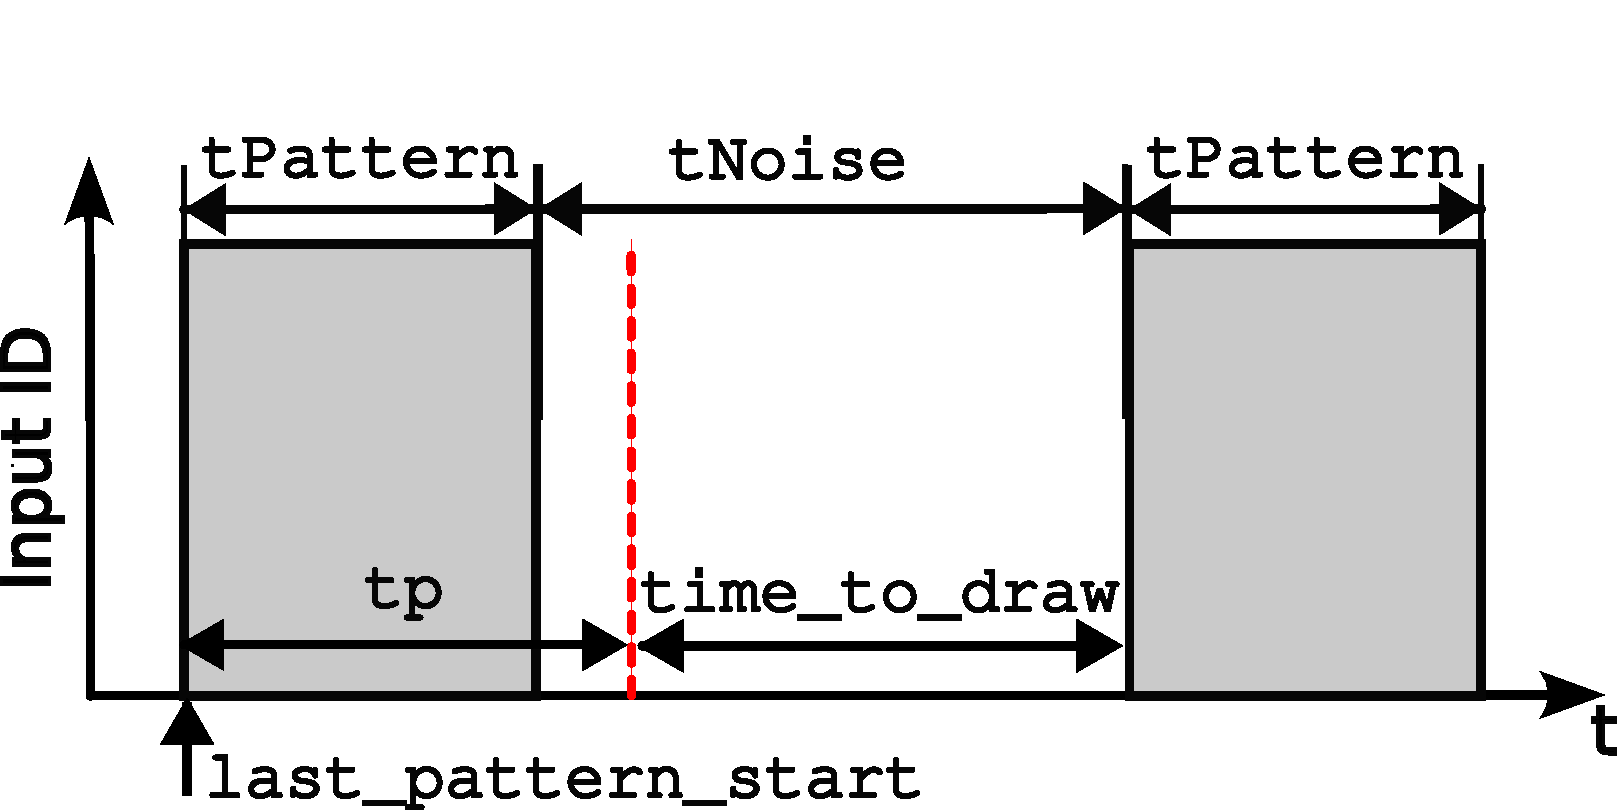
\includegraphics[width=0.9\columnwidth]{Figures/input_generator.pdf}
  \caption{Pattern Input Generation}
  \label{fig:input_generator}
\end{figure}

% Snippets
% Each input is connected to all neurons
% For more elaborate tasks pattern\_sequences are the way to go

\section{Dynamic Network Behaviour} \label{sec:dynamic_network_behaviour}
Now that the foundations of the network have been explained, it is time to dive into the actual dynamics which implement the models of plasticity and with them the ability of sequential learning. The cornerstone for neuron dynamics is the rule for determining the current membrane potential $u_k(t)$ of neuron $z_k$ (excluding the effect of lateral inhibition, which is added in \ref{eqn:firing_rate_paper}):
\begin{equation}
    u_k(t)=\sum_{i=1}^{n} w_{ki}y_i(t) + w_{k0}.
    \label{eqn:membrane_potential}
\end{equation}
Here $w_{ki}$ is the synaptic weight of an input synapse to neuron $z_k$ from pre-synaptic neuron $y_i$, and $w_{k0}$ is a bias parameter of the $k$-th neuron. This parameter has, however, no effect on the membrane potential in the implementation since it is initially set to zero and never updated. It is therefore ignored for the rest of this thesis. Finally, $y_i(t)$ fittingly denotes the current value for the excitatory postsynaptic potential (EPSP) of presynaptic neuron $y_i$. This potential is modelled as an $\alpha$-shaped kernel with rise time constant $\tau_{\text{rise}}=\SI{2}{ms}$ and decay time constant $\tau_{\text{decay}}=\SI{20}{ms}$ as follows:
\begin{equation}
    y_i(t)= \underset{t_p}{\sum} \exp\left(-\frac{t-t_p}{\tau_{\text{decay}}}\right) - exp\left(-\frac{t-t_p}{\tau_{\text{rise}}}\right)
    \label{eqn:epsp}
\end{equation}
\begin{equation*}
    \left(= \underbrace{\underset{t_p}{\sum} \exp\left(-\frac{t-t_p}{\tau_{\text{decay}}}\right)}_{\approx\texttt{epsp}} - \underbrace{\underset{t_p}{\sum} exp\left(-\frac{t-t_p}{\tau_{\text{rise}}}\right)}_{\approx\texttt{epsp2}}\right)
\end{equation*}
where $t_p$ is the set of presynaptic spike times at time $t$. This EPSP is also implemented somewhat differently from the mathematical description in Equation \ref{eqn:epsp}, which is why it was decided here to add the conversed equation for $y_i(t)$ in braces. As pointed out there, the parts of the conversed equation are realized in the code by the two variables \texttt{epsp} and \texttt{epsp2}, standing for the current EPSP values when solely considering the EPSP resulting from decay and rise respectively. While they serve the same purpose as their representations in the equation they work differently. Essentially, each of these ESPS variables decrease over time by 
\begin{equation}
    \texttt{epsp}_t=\texttt{esps}_{t-1} \left(1-\frac{\texttt{dt}}{\texttt{tau}} \right)
    \label{eqn:epsp_update}
\end{equation}
with \texttt{dt}=0.001 the simulation time step in seconds and \texttt{tau} the time constant of the \texttt{epsp} (either $\tau_{\text{rise}}$ or $\tau_{\text{decay}}$). With the decrease in EPSP for the rise and decay phases explained this still leaves the EPSP-increasing behavior undescribed. Although this is not directly mentioned in \parencite{klampfl_maass_2013}, this is in fact done by the STP mechanic described in the paper, which is why this will be further discussed in Section \ref{ssec:stp}. All that will be said about this here is that in the case of an incoming spike, the EPSP for both \texttt{epsp} and \texttt{epsp2} will be updated by $\Delta \texttt{epsp}=u\cdot R$ in addition to the EPSP decreasing behavior with $u,R\in[0,1]$ being dynamic variables that are defined in Equation \ref{eqn:stp}. 

%In the original implementation code most attributes that need to be defined per neuron or synapse (like weight and membrane potential) are handled using large arrays

\subsection{STP} \label{ssec:stp}
STP is a form of plasticity that changes the efficacy of a synapse on the scale of a few hundred to thousands of milliseconds \parencite{stevens_wang_1995}. It can be further categorized into Short-Term Facilitation (STF) and Short-Term Depression (STD) and generally causes the strength of an incoming spike to be determined also by the previous recently incoming spikes, instead of simply the synaptic weight.\\
As is clear from Equations \ref{eqn:membrane_potential} and \ref{eqn:firing_rate_paper}, there are two options in the current model to manipulate the dynamics of firing rates: using synaptic weights or EPSPs. Because STP only temporarily changes the synaptic efficacy, it makes more sense to implement it by manipulating EPSPs, which is what happens in \parencite{klampfl_maass_2013}. They determine the amplitude $A_k$ of the $k$-th input spike as follows:
\begin{equation}
\begin{aligned}
    A_k &= w_k \cdot \overbrace{u_k \cdot R_k}^{=\Delta\texttt{epsp}}\\
    u_k &= U + u_{k-1}(1-U)\exp(-\Delta_{k-1}/F)\\
    R_k &= 1 + (R_{k-1} - u_{k-1}R_{k-1}-1)\exp(-\Delta_{k-1}/D)\\
\end{aligned}
\label{eqn:stp}
\end{equation}
It is important to define the notion of "amplitude" more clearly here. Amplitude in this context refers to a combined metric of synaptic weight and EPSP associated with each given spike. The EPSP that is calculated by $u_k\cdot R_k$ was already introduced when describing the EPSP in Equation \ref{eqn:epsp} and is responsible for the EPSP increase on spike input.\\
The interspike intervals of the entire spike train up to the $k$-th spike are given by $\Delta_1, \Delta_2, \dots, \Delta_{k-1}$, while $D$ and $F$ are STD- and STF-related time parameters. $U$, $D$ and $F$ all have in common that they are set randomly for each synapse from Gaussian distributions $\mathcal{N}(\mu, \sigma^2)$ with $\sigma=0.5\mu$ and $\mu_U=0.5$, $\mu_D=0.11$, $\mu_F=0.005$. In the implementation the additional constraints $U\geq 0$, $D,F\geq \texttt{dt}$ are added to ensure that the amplitude does not take on unintended values.\\
% [describe the effect of this plasticity rule]
Klampfl and Maass stated they adopted this short-term plasticity model from \parencite{markram_wang_tsodyks_1998}. However, on comparison, it is noticeable a detail was altered when doing so. Instead of the definition of $R_k$ from Equation \ref{eqn:stp}, the following definition  would conform with their cited model:
\begin{equation*}
    R_k = 1 + (R_{k_1} - \mathbf{u_{k}}R_{k-1}-1)\exp(-\Delta_{k-1}/D)
\end{equation*}
with $u_k$ instead of $u_{k-1}$. It is unclear if this detail has any significant effect and if it was an intentional decision that was simply not explained by Klampfl and Maass, but it is worth mentioning and should be considered when using their model for future work.\\
Another mistake of the computational kind was also found in the original implementation. Usually, only recurrent connections should be subject to STP, but due to an error in the calculation of $R_k$, STP was partially applied to input connections as well.


\subsection{STDP} \label{ssec:stdp}

STDP, unlike STP, is a long-term plasticity that is based on temporal differences between pre- and post-spikes. More precisely, this means that whenever a postsynaptic neuron $z$ emits a spike at time $t_{post}$ and receives an incoming spike from presynaptic neuron $y$ at time $t_{pre}$, then the weight of the connecting synapse is increased if $t_{pre}< t_{post}$ and decreased if $t_{pre}\geq t_{post}$. There are many different rules that model STDP, but Klampfl and Maass stated they wanted to implement it using the following weight update rule:
\begin{equation}
    \Delta w_{ki}=y_i(t) \cdot c \cdot e^{-w_{ki}} - 1 = \frac{c\cdot y_i(t)-e^{w_{ki}}}{e^{w_{ki}}},
    \label{eqn:stdp_paper}
\end{equation}
where $w_{ki}$ denotes the weight of the synapse input to neuron $z_k$ from pre-synaptic neuron $y_i$. This weight update should be performed every time neuron $z_k$ fires. Furthermore, $y_i(t)$ denotes the current value of the EPSP at presynaptic neuron $y_i$ as formulated in Equation \ref{eqn:epsp} and $c$ is a scaling parameter used to keep the synaptic weights in a positive range. This parameter is comprised of the learning rate $\eta^*=0.05$ and an offset of $5$ like this: $c=0.05 \cdot \exp(5)=7.42$.\\
Obviously, this STDP model does not make use of $t_{pre}$ and $t_{post}$ directly, which is somewhat unusual. It rather exploits the fact that the EPSP $y_i(t)$ of the presynaptic neuron should be high if it has recently spiked, and low if it has not spiked in the recent past. To better visualize STDP a common way is to plot an STDP window. STDP windows can be created practically by setting a fixed spike time for the post-spike of a neuron and confronting it with varying pre-spike times. For each pre-/post-spike combination, the resulting weight change is plotted. For the STDP rule from Equation 5 of \parencite{klampfl_maass_2013} this produces the STDP window in Figure \ref{fig:stdp_window}. 
As illustrated there, the weight is reduced by a constant of $-1$ every time a pre-spike arrives earlier than the post-spike is emitted and is only ever increased if the pre-spike comes in later, but only for a brief period of time.\\
\begin{figure}[htbp]
    \centering
    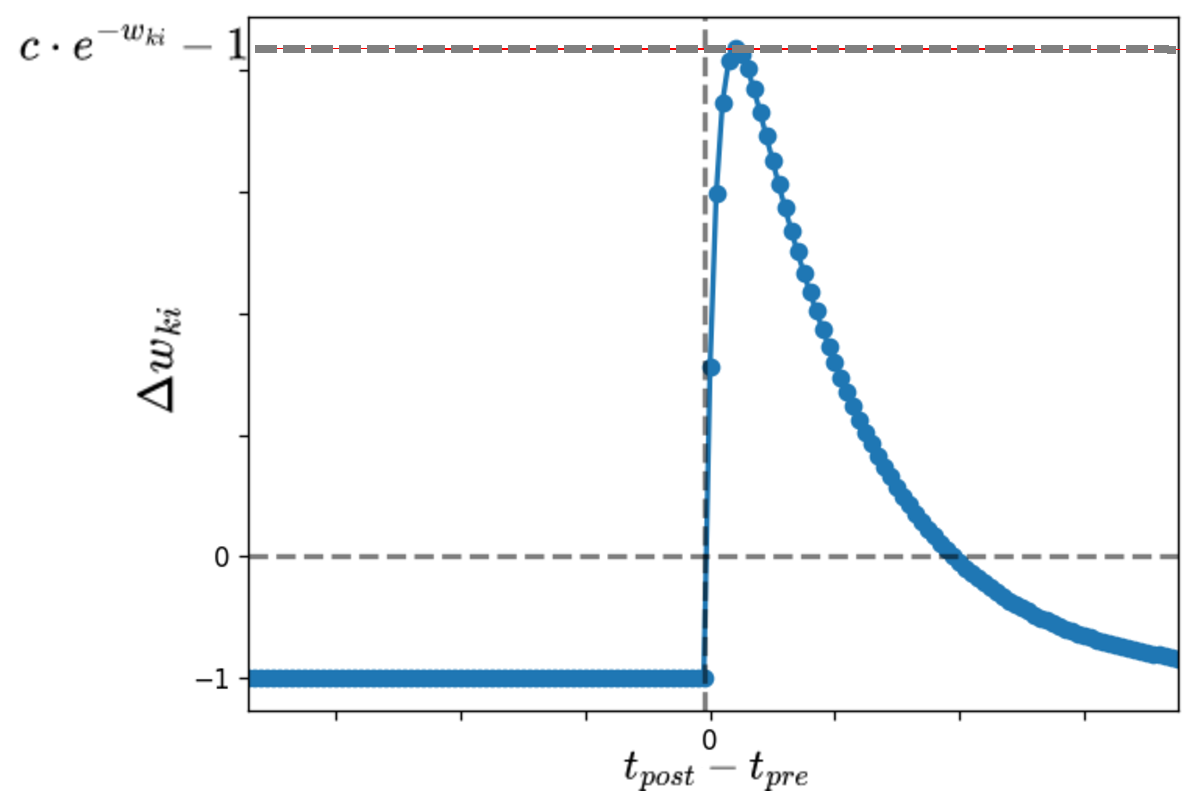
\includegraphics[width=0.7\columnwidth]{Figures/stdp_window.pdf}
    \caption{STDP window}
    \label{fig:stdp_window}
\end{figure}
\\ \ \\ % [TODO: STDP window from paper]
% [maybe TODO: explain STDP window above]
It is also claimed in the original paper that the bias parameter from Equation \ref{eqn:membrane_potential} is updated by the following rule:
\begin{equation*}
    \Delta w_{k0} = 
    \begin{cases}
        c\cdot e^{-w_{k0}} -1 & \text{if neuron } z_k \text{ fires}\\
        -1 & \text{else}
    \end{cases}
\end{equation*}
However, this could not be found in the implementation code, which is why it will not be regarded for the replication. Apart from this, the actual implementation of $\Delta w_{ki}$ also seems to deviate slightly from Equation \ref{eqn:stdp_paper}:
\begin{equation}
    \Delta w_{ki} = \eta_{ki} \cdot \frac{y_i(t)-e^{w_{ki}}}{\max \{e^{w_{ki}}, \eta_{ki}\}}
    \label{eqn:stdp_real}
\end{equation}
The reason for this is that Klampfl and Maass decided to also adopt adaptive learning rates for synapses from \parencite{nessler_et_al_2013}. This is handled by the synapse-specific learning rate $\eta_{ki}$, which replaces the static parameter $c$.

\subsubsection{Variance Tracking} \label{sec:variance_tracking}
The integration of adaptive learning rates is done by a heuristic called variance tracking, described in \parencite{nessler_et_al_2013}. Its purpose is to facilitate the spontaneous reorganization of the learned models (encoded in the form of synaptic weights) in the event that the input distribution $p^*(\mathbf{y})$ changes. The input distribution $p^*(\mathbf{y})$ would for example change when a new different spike pattern would be presented to the network for learning.\\
This variance tracking is defined in Equation 71 of \parencite{nessler_et_al_2013}:
\begin{equation}
    \eta_{ki}^{new} = \frac{ \text{E}[w_{ki}^2] - \text{E}[w_{ki}]^2 }{ e^{-\text{E}[w_{ki}]} + 1 } 
    = \frac{ \text{Var}(w_{ki}) }{ e^{-\text{E}[w_{ki}]} + 1 },
    \label{eqn:variance_tracking}
\end{equation}
which is used to calculate $\eta_{ki}=\eta^*\cdot \eta_{ki}^{new}$. In the following let $S_{ki}:=\text{E}[w_{ki}]$ and $Q_{ki}:=\text{E}[w_{ki}^2]$, as these variables are used in the original implementation. The way their values are determined there is by summing over the presynaptic spike times $t_p$ of their associated synapse up to the current point in time:
\begin{equation}
\begin{aligned}
    S_{ki}^{(t)} &= \sum_{t_p}^t \eta_{ki}^{(t_p)} \cdot (w_{ki}^{(t_p)}-S_{ki}^{(t_p)})\\
    Q_{ki}^{(t)} &= \sum_{t_p}^t \eta_{ki}^{(t_p)} \cdot (w_{ki}^2 {}^{(t_p)}-Q_{ki}^{(t_p)})\\
    \text{with } S^{(0)}&=0 \text{ and } Q^{(0)}=1
\end{aligned}
\label{eqn:variance_tracking_2}
\end{equation}

\section{Summary of Complications} \label{sec:summary_complications_original}
While working on this thesis, several major obstacles were encountered. Those specific to the paper and the associated code base are briefly summarized in this section for better outlining of difficult problems to avoid future issues.
\begin{itemize}
    \item The rates described in the paper differ from the implementation. This is further discussed in Section \ref{sec:input_generation}.
    \item Despite what the paper states about neurons being individually connected with probability $p(d)$, in the code only entire WTAs are connected to each other with all-to-all connections between their respective sets of neurons.
    \item As discussed in Section \ref{ssec:stdp}, the actual implementation of STDP differed clearly from the description in the paper.
    \item There was also an implementation error in the STP, where STP was partially applied to input synapses, which is not intended (mentioned in Section \ref{ssec:stp})
    \item The used STP rule in both paper and code is adopted incorrectly from the cited source in the paper (see Section \ref{ssec:stp})
\end{itemize}

% Snippets
% it was found that variance tracking is necessary

% list of important parameters that will be referenced e.g. when producing readouts for the network

